This section discusses the various details about software implemented in detail.

\section{Design}

The software is implemented in Java using ArangoDB as the backend database. The application has 3 layer structure as per Figure \ref{fig:appdesign}. The database layer which is the ArangoDB database itself. The business layer, this layer contains all the logic for talking to the backend ArangoDB, the clustering algorithms and other functions. The application has 2 frontends: Web application which is made using the Spring framework in Java and a simple command line application. Both the front end uses the same business layer hence providing the same functionality. 

The way this project was strategised was to make command line first for easy testing of the core functionality like clustering, inserting the data, getting the data etc. Then the same core libraries are called via the web application. The web application was created for ease of use and multiple simultaneous analysis. Another reason for keeping the command line application was, some of the commands took too long to process. The connection between the server and the client used to timeout. Web sockets helped to keep the connection alive but once the connection is broken the results were lost in the process.

The whole project has 3 modules namely core, cmdapp, webapp. Gradle build tool was used for compiling, testing and running the application. 

\begin{figure}[ht]
    \centering
    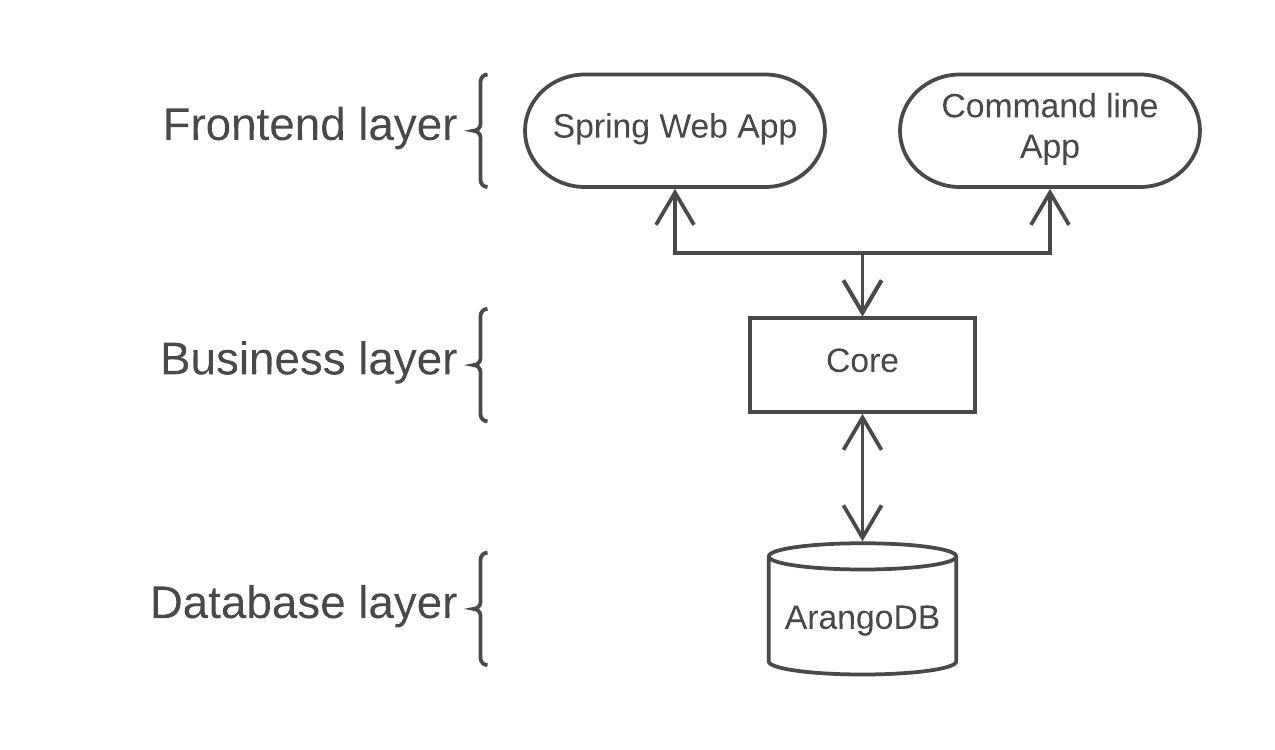
\includegraphics[width=300pt]{appdesign}
    \caption{\label{fig:appdesign} Structure of the app}
\end{figure}

\subsection{ArangoDB}

ArangoDB is a multi-model database. It supports three data models namely key/value, documents, graphs and a unified query language called AQL. AQL is very similar to SQL query language. AQL is used for CRUD operations. It provides scalable and highly efficient queries. It uses JSON as a default storage schema. 

The application uses this database for all the heavy duty data operations like grouping, summing, filtering neighbours etc. The reason a database was used instead of doing it directly in Java was for faster development, thread-safety and also the indexes provided by the database for faster queries. 

\subsection{Core}

This business layer of the application contains all the core logic. It contains all the query, the driver to talk to ArangoDB, the logic for converting from and to CSV etc. The core module uses spring-context which is an application IoC (Inversion of Control) container. This container can be consumed by any application by adding the library and providing the database connection configuration. This saves the other application from creating each and every object. The IoC container creates the object for the application automatically at runtime. The strategy was to create a library which contains all main logic and which can be consumed by any kind of application. This can be seen as we have implemented in two applications command line and web application.

\begin{figure}[!ht]
    \centering
    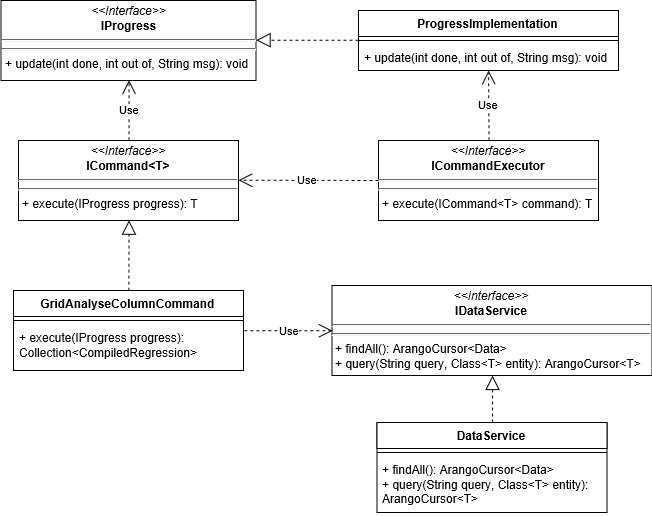
\includegraphics[width=400pt]{umlcore}
    \caption{\label{fig:umlcore} UML diagram of the command pattern in the core module}
\end{figure}

Apart from using IoC containers, the main design pattern used by this module of application is the Command Pattern\cite{dupire2001command}. In this pattern, an object is encapsulated with all the information needed to perform an action. The biggest feature of the command pattern is that it can be executed at any point in time. The command in our case is executed by a Command executor. This separation of the actual command and executor allows for greater changes in the future of the project. It provides a lot of flexibility and ease of adding and replacing commands in later stages of the development. One of the purposes of using command pattern was the certain routines in the application are quite slow e.g. distance-based clustering. The command pattern creates a unified way for getting the updates/progress of a task being executed.

The drawbacks of this pattern are it makes the source code larger quickly because one file can only represent one command. The number of files in the project increases very quickly. Command names are usually big and so goes for the file names. The order of commands becomes important at later stages and can jeopardize the reliability of the system\cite{dupire2001command}.

Figure\ref{fig:umlcore}, shows the implementation of command pattern. Only one Concrete command (GridAnalyseColumnCommand) is been shown. There are various commands implemented for data insertion, data deletion, distance-based analysing etc. It can be seen from the figure\ref{fig:umlcore} that no implementation is defined for ICommandExecutor. This is because the modules consuming this core module library can implement according to their need. Similarly, for the IProgress, modules can implement their own version depending on their type of the application. The parameters of the command are supplied when creating the instance of the object. The command object constructor contains all the necessary arguments needed for execution at a later stage.

\subsection{Webapp}

The web application is built on Spring framework. It comes with IoC container which can easily pass in the database connection to the core library being consumed. In this module, the progress and command executor interfaces are implements to the needs of the web application. The progress interface implementation uses WebSocket for sending the update of how much work has been completed by the command. WebSocket is full-duplex communication channel over TCP which allows server and client to send messages to each other asynchronously.

The application maps the REST APIs to the Commands in the core module. The UI of the web application uses AngularJS which is a client-side front-end web framework. AngularJS framework allows to makes calls to the REST Endpoints and also act accordingly to the messages received by the server through WebSocket.

\subsection{Command Line}

The command line application also uses the core module to do a similar task. The mapping is from command line arguments to core module's command. In this module, as well a different implementation is done for the progress and command executor interfaces because this time the display and execution are in the command line. Since the core module uses IoC container. Spring-context was added and application context was created at the start of the application. The arguments were parsed via the JCommander library. 

\section{Optimizations}

In this section, we discuss Optimizations that were done to speed up the computations.

\subsection{Grid clustering algorithm}

As per the pseudocode~\ref{alg:gridExistence}, it can be seen that the Time complexity is \(O(N\log(N))\) which was due to the sorting performed on the coordinate of the box calculated for each data point. But as one can see from the pseudo code the two \(N\) iterations were performed. First, for calculating the coordinate of the \(k-cube\) they belong to and then for the grouping the data points into the result. This result is then used for either finding violation of functional relation or for analysing the relation between the parameters. 

The two extra \(N\) iterations were optimised by the ArangoDB by dividing the 3 iterations into 2 nodes. The first node sorts the data points by calculating the coordinates of the \(k-cube\) on the go and attaching it temporarily to the dataset for reuse if the data set is accessed again by the sort. After sorting the data points with its coordinates are send to the second node. The second node then groups the data on the fly as the groups are accessed. This is because the all the groups with equal coordinate lies next to each other. The groups and the data coming from the second node is pipelined to our computations that are performed on the nodes. 

It is impossible to parallelize this algorithm because of its aggregating nature, where one point cannot be in more than one cluster. But due to its \(O(N\log(N))\) complexity, overall the algorithm is quite fast and linear.

\subsection{Distance based clustering}

In the distance based clustering~\ref{alg:dbscanExistence}, we calculated the time complexity to be \(O(N^2)\). This was due to nature of the algorithm to find neighbouring data points for every data point in the dataset. 

It is not possible to reduce the first outer iteration, as we have to go through each data point for analysing the whole dataset. The second one, it is not required to go through the entire data points as long as we can find all the points that are close to each other within some tolerance. This makes it possible for optimisations. One of the approaches is to save \(N^2\) distances between each and every data point and then making it easier for all the subsequent queries. This is very practical and blazingly fast as only one time, a slow operation is required for saving all the distances between each and every point. Then finding neighbours is a trivial task of going through the entire edges and getting all those points where the distance is less than the specified tolerance. This is practical for smaller dataset but due to the square space complexity. But as the number of records gets larger it becomes inefficient to not only run the one-time insertion but also storing the same.

So, another way was chosen in which indexes were created to fasten the search to find the neighbours. We filter the data with conditions such that data points whose possibility of becoming neighbour is zero are filtered before the distance is actually and calculate and confirmed.

We use the fact that \(dist(v, u) \geq 0\) always where \(v, u\) are two data points vectors in space. 

Let the \(tol\) be the max distance (tolerance) allowed between two data points. 
Let \(u\) be the data point vector with dimension \(k\) whose neighbours are to be found.
Let \(v\) be any vector in the dataset.

Then for any value of:
\[v[i] > u[i] + tol \vee v[i] < u[i] - tol\] where \(i \in [0, k-1]\)
\[\implies dist(u, v) > tol\]

The reason is if any one of the values in vector \(v\) is more than \(tol\) units away then because the distance is added from all the other values of the vector as well. The total distance will definitely be more than \(tol\).

But this filtering method is still not good as we still have to go through all the dataset to check whether any of the value is greater than \(tol\) or not. ArangoDB provides APIs to create indexes on the fields of documents for faster access to documents. It provides many different types of indexes such as Hash index, skip-list index, full-text index etc. Each index uses a special data structure to fasten different types of searches. As we are interested in range based queries. Skip list comes into play. Skiplist maintains a separate linked hierarchy of ordered values. They fasten up the equality lookups, range queries and sorting. The skip-list is added on to every parameter of the dataset and then when the filtering out condition is used before calculating the distance. The number of iteration will drop from \(N\) to the \(Amortised-N\).

Another performance improvement that is done is by parallelising the outer loops. As ArangoDB supports multiple reads at the same time and the inner loop has no dependency on other iteration. The outer loop is parallelised which further decreases the running time by the number of threads the CPU can handle at a time. 

\section{Testing}

All the functionality in core module has been well tested using the JUnit framework. Unit tests were created for classes which did not have external dependencies whereas Integration tests were created for classes that depended on other modules such as Commands, Data service etc. The reason unit test was not preferred because the unit test requires mocking of all of its dependencies. Integration test was preferred because it gave more confidence that the system works correctly as a whole. For components like analyse parameter etc, integration tests were created. Test data was entered directly into the database and commands were then called, asserting the results by the commands. Integration testing is not chosen for larger projects as these tests are very much slower than the unit test. But because our project involves a lot of database queries and is not at scale with industrial software, integration tests were performed. 

Tests were created for almost every component and module. Rigorous testing was performed on core modules. As this module contains all the logic and interaction to the database. For parts such as clustering, regression, small records were created whose result we knew. These small records were entered into the database and clustering algorithms were called such that it gives the output known already. The testing is more of the black box testing form. A number of small hand-made datasets and their known output is used to test the components.